\documentclass[1p]{elsarticle_modified}
%\bibliographystyle{elsarticle-num}

%\usepackage[colorlinks]{hyperref}
%\usepackage{abbrmath_seonhwa} %\Abb, \Ascr, \Acal ,\Abf, \Afrak
\usepackage{amsfonts}
\usepackage{amssymb}
\usepackage{amsmath}
\usepackage{amsthm}
\usepackage{scalefnt}
\usepackage{amsbsy}
\usepackage{kotex}
\usepackage{caption}
\usepackage{subfig}
\usepackage{color}
\usepackage{graphicx}
\usepackage{xcolor} %% white, black, red, green, blue, cyan, magenta, yellow
\usepackage{float}
\usepackage{setspace}
\usepackage{hyperref}

\usepackage{tikz}
\usetikzlibrary{arrows}

\usepackage{multirow}
\usepackage{array} % fixed length table
\usepackage{hhline}

%%%%%%%%%%%%%%%%%%%%%
\makeatletter
\renewcommand*\env@matrix[1][\arraystretch]{%
	\edef\arraystretch{#1}%
	\hskip -\arraycolsep
	\let\@ifnextchar\new@ifnextchar
	\array{*\c@MaxMatrixCols c}}
\makeatother %https://tex.stackexchange.com/questions/14071/how-can-i-increase-the-line-spacing-in-a-matrix
%%%%%%%%%%%%%%%

\usepackage[normalem]{ulem}

\newcommand{\msout}[1]{\ifmmode\text{\sout{\ensuremath{#1}}}\else\sout{#1}\fi}
%SOURCE: \msout is \stkout macro in https://tex.stackexchange.com/questions/20609/strikeout-in-math-mode

\newcommand{\cancel}[1]{
	\ifmmode
	{\color{red}\msout{#1}}
	\else
	{\color{red}\sout{#1}}
	\fi
}

\newcommand{\add}[1]{
	{\color{blue}\uwave{#1}}
}

\newcommand{\replace}[2]{
	\ifmmode
	{\color{red}\msout{#1}}{\color{blue}\uwave{#2}}
	\else
	{\color{red}\sout{#1}}{\color{blue}\uwave{#2}}
	\fi
}

\newcommand{\Sol}{\mathcal{S}} %segment
\newcommand{\D}{D} %diagram
\newcommand{\A}{\mathcal{A}} %arc


%%%%%%%%%%%%%%%%%%%%%%%%%%%%%5 test

\def\sl{\operatorname{\textup{SL}}(2,\Cbb)}
\def\psl{\operatorname{\textup{PSL}}(2,\Cbb)}
\def\quan{\mkern 1mu \triangleright \mkern 1mu}

\theoremstyle{definition}
\newtheorem{thm}{Theorem}[section]
\newtheorem{prop}[thm]{Proposition}
\newtheorem{lem}[thm]{Lemma}
\newtheorem{ques}[thm]{Question}
\newtheorem{cor}[thm]{Corollary}
\newtheorem{defn}[thm]{Definition}
\newtheorem{exam}[thm]{Example}
\newtheorem{rmk}[thm]{Remark}
\newtheorem{alg}[thm]{Algorithm}

\newcommand{\I}{\sqrt{-1}}
\begin{document}

%\begin{frontmatter}
%
%\title{Boundary parabolic representations of knots up to 8 crossings}
%
%%% Group authors per affiliation:
%\author{Yunhi Cho} 
%\address{Department of Mathematics, University of Seoul, Seoul, Korea}
%\ead{yhcho@uos.ac.kr}
%
%
%\author{Seonhwa Kim} %\fnref{s_kim}}
%\address{Center for Geometry and Physics, Institute for Basic Science, Pohang, 37673, Korea}
%\ead{ryeona17@ibs.re.kr}
%
%\author{Hyuk Kim}
%\address{Department of Mathematical Sciences, Seoul National University, Seoul 08826, Korea}
%\ead{hyukkim@snu.ac.kr}
%
%\author{Seokbeom Yoon}
%\address{Department of Mathematical Sciences, Seoul National University, Seoul, 08826,  Korea}
%\ead{sbyoon15@snu.ac.kr}
%
%\begin{abstract}
%We find all boundary parabolic representation of knots up to 8 crossings.
%
%\end{abstract}
%\begin{keyword}
%    \MSC[2010] 57M25 
%\end{keyword}
%
%\end{frontmatter}

%\linenumbers
%\tableofcontents
%
\newcommand\colored[1]{\textcolor{white}{\rule[-0.35ex]{0.8em}{1.4ex}}\kern-0.8em\color{red} #1}%
%\newcommand\colored[1]{\textcolor{white}{ #1}\kern-2.17ex	\textcolor{white}{ #1}\kern-1.81ex	\textcolor{white}{ #1}\kern-2.15ex\color{red}#1	}

{\Large $\underline{12a_{0195}~(K12a_{0195})}$}

\setlength{\tabcolsep}{10pt}
\renewcommand{\arraystretch}{1.6}
\vspace{1cm}\begin{tabular}{m{100pt}>{\centering\arraybackslash}m{274pt}}
\multirow{5}{120pt}{
	\centering
	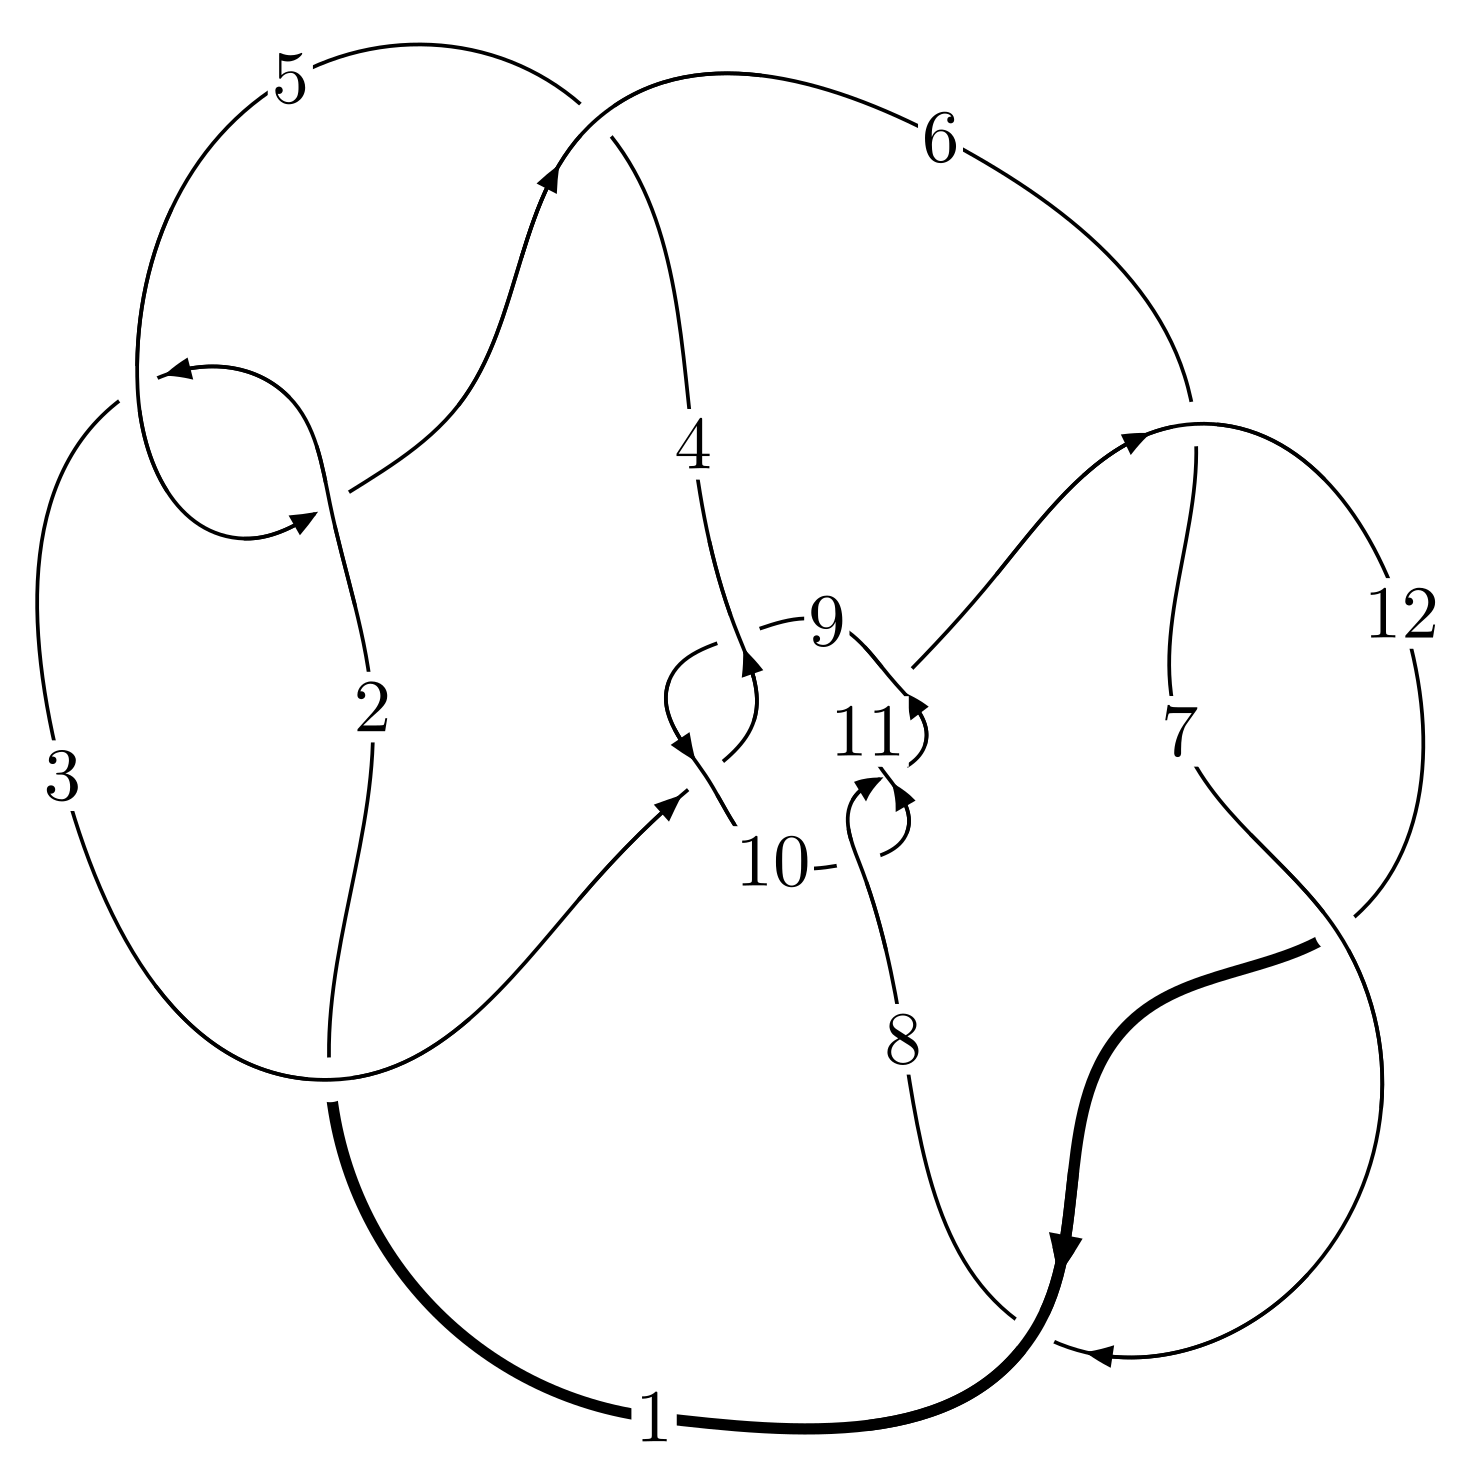
\includegraphics[width=112pt]{../../../GIT/diagram.site/Diagrams/png/996_12a_0195.png}\\
\ \ \ A knot diagram\footnotemark}&
\allowdisplaybreaks
\textbf{Linearized knot diagam} \\
\cline{2-2}
 &
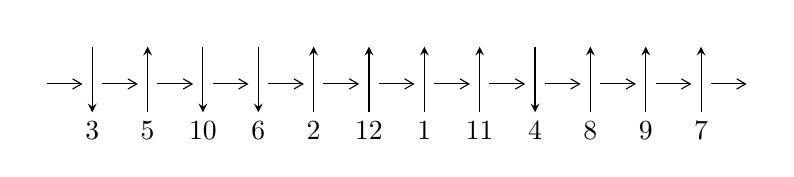
\begin{tikzpicture}[x=20pt, y=17pt]
	% nodes
	\node (C0) at (0, 0) {};
	\node (C1) at (1, 0) {};
	\node (C1U) at (1, +1) {};
	\node (C1D) at (1, -1) {3};

	\node (C2) at (2, 0) {};
	\node (C2U) at (2, +1) {};
	\node (C2D) at (2, -1) {5};

	\node (C3) at (3, 0) {};
	\node (C3U) at (3, +1) {};
	\node (C3D) at (3, -1) {10};

	\node (C4) at (4, 0) {};
	\node (C4U) at (4, +1) {};
	\node (C4D) at (4, -1) {6};

	\node (C5) at (5, 0) {};
	\node (C5U) at (5, +1) {};
	\node (C5D) at (5, -1) {2};

	\node (C6) at (6, 0) {};
	\node (C6U) at (6, +1) {};
	\node (C6D) at (6, -1) {12};

	\node (C7) at (7, 0) {};
	\node (C7U) at (7, +1) {};
	\node (C7D) at (7, -1) {1};

	\node (C8) at (8, 0) {};
	\node (C8U) at (8, +1) {};
	\node (C8D) at (8, -1) {11};

	\node (C9) at (9, 0) {};
	\node (C9U) at (9, +1) {};
	\node (C9D) at (9, -1) {4};

	\node (C10) at (10, 0) {};
	\node (C10U) at (10, +1) {};
	\node (C10D) at (10, -1) {8};

	\node (C11) at (11, 0) {};
	\node (C11U) at (11, +1) {};
	\node (C11D) at (11, -1) {9};

	\node (C12) at (12, 0) {};
	\node (C12U) at (12, +1) {};
	\node (C12D) at (12, -1) {7};
	\node (C13) at (13, 0) {};

	% arrows
	\draw[->,>={angle 60}]
	(C0) edge (C1) (C1) edge (C2) (C2) edge (C3) (C3) edge (C4) (C4) edge (C5) (C5) edge (C6) (C6) edge (C7) (C7) edge (C8) (C8) edge (C9) (C9) edge (C10) (C10) edge (C11) (C11) edge (C12) (C12) edge (C13) ;	\draw[->,>=stealth]
	(C1U) edge (C1D) (C2D) edge (C2U) (C3U) edge (C3D) (C4U) edge (C4D) (C5D) edge (C5U) (C6D) edge (C6U) (C7D) edge (C7U) (C8D) edge (C8U) (C9U) edge (C9D) (C10D) edge (C10U) (C11D) edge (C11U) (C12D) edge (C12U) ;
	\end{tikzpicture} \\
\hhline{~~} \\& 
\textbf{Solving Sequence} \\ \cline{2-2} 
 &
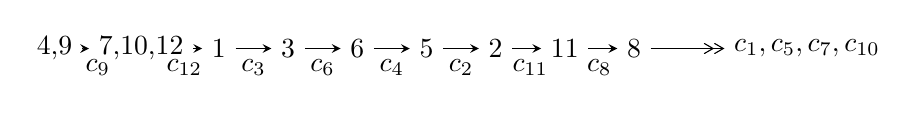
\begin{tikzpicture}[x=25pt, y=7pt]
	% node
	\node (A0) at (-1/8, 0) {4,9};
	\node (A1) at (9/8, 0) {7,10,12};
	\node (A2) at (9/4, 0) {1};
	\node (A3) at (13/4, 0) {3};
	\node (A4) at (17/4, 0) {6};
	\node (A5) at (21/4, 0) {5};
	\node (A6) at (25/4, 0) {2};
	\node (A7) at (29/4, 0) {11};
	\node (A8) at (33/4, 0) {8};
	\node (C1) at (1/2, -1) {$c_{9}$};
	\node (C2) at (7/4, -1) {$c_{12}$};
	\node (C3) at (11/4, -1) {$c_{3}$};
	\node (C4) at (15/4, -1) {$c_{6}$};
	\node (C5) at (19/4, -1) {$c_{4}$};
	\node (C6) at (23/4, -1) {$c_{2}$};
	\node (C7) at (27/4, -1) {$c_{11}$};
	\node (C8) at (31/4, -1) {$c_{8}$};
	\node (A9) at (43/4, 0) {$c_{1},c_{5},c_{7},c_{10}$};

	% edge
	\draw[->,>=stealth]	
	(A0) edge (A1) (A1) edge (A2) (A2) edge (A3) (A3) edge (A4) (A4) edge (A5) (A5) edge (A6) (A6) edge (A7) (A7) edge (A8) ;
	\draw[->>,>={angle 60}]	
	(A8) edge (A9);
\end{tikzpicture} \\ 

\end{tabular} \\

\footnotetext{
The image of knot diagram is generated by the software ``\textbf{Draw programme}" developed by Andrew Bartholomew(\url{http://www.layer8.co.uk/maths/draw/index.htm\#Running-draw}), where we modified some parts for our purpose(\url{https://github.com/CATsTAILs/LinksPainter}).
}\phantom \\ \newline 
\centering \textbf{Ideals for irreducible components\footnotemark of $X_{\text{par}}$} 
 
\begin{align*}
I^u_{1}&=\langle 
2.98338\times10^{44} u^{32}+6.07211\times10^{44} u^{31}+\cdots+8.30969\times10^{46} d+2.51360\times10^{46},\\
\phantom{I^u_{1}}&\phantom{= \langle  }7.43844\times10^{44} u^{32}+1.59524\times10^{45} u^{31}+\cdots+1.66194\times10^{47} c-9.07104\times10^{46},\\
\phantom{I^u_{1}}&\phantom{= \langle  }-2.43633\times10^{45} u^{32}-5.73801\times10^{45} u^{31}+\cdots+8.30969\times10^{46} b-1.04987\times10^{47},\\
\phantom{I^u_{1}}&\phantom{= \langle  }-1.26296\times10^{45} u^{32}-3.00101\times10^{45} u^{31}+\cdots+8.30969\times10^{46} a-1.12331\times10^{47},\\
\phantom{I^u_{1}}&\phantom{= \langle  }u^{33}+3 u^{32}+\cdots-32 u-32\rangle \\
I^u_{2}&=\langle 
-33577974480092 u^{24} a+53309187006291 u^{24}+\cdots+196002507777016 a+140186694789454,\\
\phantom{I^u_{2}}&\phantom{= \langle  }-106618374012582 u^{24} a-153454383700573 u^{24}+\cdots-280373389578908 a-552236032471050,\\
\phantom{I^u_{2}}&\phantom{= \langle  }b-1,\;-1.33548\times10^{14} a u^{24}+1.93299\times10^{14} u^{24}+\cdots+1.95694\times10^{15} a+2.03280\times10^{15},\\
\phantom{I^u_{2}}&\phantom{= \langle  }u^{25}- u^{24}+\cdots+4 u+4\rangle \\
\\
I^v_{1}&=\langle 
a,\;d,\;c-1,\;b-1,\;v^2- v+1\rangle \\
I^v_{2}&=\langle 
a,\;d+1,\;c+a,\;b-1,\;v^2- v+1\rangle \\
I^v_{3}&=\langle 
a,\;d+1,\;c+a+1,\;b-1,\;v+1\rangle \\
I^v_{4}&=\langle 
c,\;d+1,\;c b+a+1,\;- v^2 b a+v^2 c- v^2 b+2 v^2 a- c v- a v+2 v^2+c- v,\;b^2 v^2-2 v^2 b+b v+v^2- v+1\rangle \\
\end{align*}
\raggedright * 5 irreducible components of $\dim_{\mathbb{C}}=0$, with total 88 representations.\\
\raggedright * 1 irreducible components of $\dim_{\mathbb{C}}=1$ \\
\footnotetext{All coefficients of polynomials are rational numbers. But the coefficients are sometimes approximated in decimal forms when there is not enough margin.}
\newpage
\renewcommand{\arraystretch}{1}
\centering \section*{I. $I^u_{1}= \langle 2.98\times10^{44} u^{32}+6.07\times10^{44} u^{31}+\cdots+8.31\times10^{46} d+2.51\times10^{46},\;7.44\times10^{44} u^{32}+1.60\times10^{45} u^{31}+\cdots+1.66\times10^{47} c-9.07\times10^{46},\;-2.44\times10^{45} u^{32}-5.74\times10^{45} u^{31}+\cdots+8.31\times10^{46} b-1.05\times10^{47},\;-1.26\times10^{45} u^{32}-3.00\times10^{45} u^{31}+\cdots+8.31\times10^{46} a-1.12\times10^{47},\;u^{33}+3 u^{32}+\cdots-32 u-32 \rangle$}
\flushleft \textbf{(i) Arc colorings}\\
\begin{tabular}{m{7pt} m{180pt} m{7pt} m{180pt} }
\flushright $a_{4}=$&$\begin{pmatrix}0\\u\end{pmatrix}$ \\
\flushright $a_{9}=$&$\begin{pmatrix}1\\0\end{pmatrix}$ \\
\flushright $a_{7}=$&$\begin{pmatrix}0.0151986 u^{32}+0.0361146 u^{31}+\cdots-0.765502 u+1.35181\\0.0293192 u^{32}+0.0690520 u^{31}+\cdots-1.79735 u+1.26343\end{pmatrix}$ \\
\flushright $a_{10}=$&$\begin{pmatrix}1\\u^2\end{pmatrix}$ \\
\flushright $a_{12}=$&$\begin{pmatrix}-0.00447577 u^{32}-0.00959870 u^{31}+\cdots+0.258096 u+0.545811\\-0.00359025 u^{32}-0.00730726 u^{31}+\cdots+0.166618 u-0.302490\end{pmatrix}$ \\
\flushright $a_{1}=$&$\begin{pmatrix}-0.0150061 u^{32}-0.0352289 u^{31}+\cdots+1.12333 u-0.0633242\\-0.0275000 u^{32}-0.0663276 u^{31}+\cdots+1.81369 u-1.26434\end{pmatrix}$ \\
\flushright $a_{3}=$&$\begin{pmatrix}u\\u^3+u\end{pmatrix}$ \\
\flushright $a_{6}=$&$\begin{pmatrix}0.0197140 u^{32}+0.0451970 u^{31}+\cdots-0.857293 u+1.51428\\0.0347201 u^{32}+0.0804259 u^{31}+\cdots-1.98062 u+1.57761\end{pmatrix}$ \\
\flushright $a_{5}=$&$\begin{pmatrix}0.0254851 u^{32}+0.0825348 u^{31}+\cdots-2.53688 u-1.85413\\0.0263436 u^{32}+0.101429 u^{31}+\cdots-2.69293 u-2.59143\end{pmatrix}$ \\
\flushright $a_{2}=$&$\begin{pmatrix}-0.0169811 u^{32}-0.0390647 u^{31}+\cdots+1.30794 u-0.509563\\-0.0254461 u^{32}-0.0623905 u^{31}+\cdots+2.00195 u-1.64373\end{pmatrix}$ \\
\flushright $a_{11}=$&$\begin{pmatrix}-0.000885519 u^{32}-0.00229144 u^{31}+\cdots+0.0914785 u+0.848301\\-0.00359025 u^{32}-0.00730726 u^{31}+\cdots+0.166618 u-0.302490\end{pmatrix}$ \\
\flushright $a_{8}=$&$\begin{pmatrix}-0.000885519 u^{32}-0.00229144 u^{31}+\cdots+0.0914785 u+0.848301\\0.00540092 u^{32}+0.0113739 u^{31}+\cdots-0.183270 u+0.314174\end{pmatrix}$\\&\end{tabular}
\flushleft \textbf{(ii) Obstruction class $= -1$}\\~\\
\flushleft \textbf{(iii) Cusp Shapes $= 0.0605080 u^{32}+0.0513753 u^{31}+\cdots+7.44134 u+11.1534$}\\~\\
\newpage\renewcommand{\arraystretch}{1}
\flushleft \textbf{(iv) u-Polynomials at the component}\newline \\
\begin{tabular}{m{50pt}|m{274pt}}
Crossings & \hspace{64pt}u-Polynomials at each crossing \\
\hline $$\begin{aligned}c_{1},c_{4}\end{aligned}$$&$\begin{aligned}
&u^{33}+11 u^{32}+\cdots+8 u-16
\end{aligned}$\\
\hline $$\begin{aligned}c_{2},c_{5}\end{aligned}$$&$\begin{aligned}
&u^{33}+u^{32}+\cdots-12 u+4
\end{aligned}$\\
\hline $$\begin{aligned}c_{3},c_{9}\end{aligned}$$&$\begin{aligned}
&u^{33}-3 u^{32}+\cdots-32 u+32
\end{aligned}$\\
\hline $$\begin{aligned}c_{6},c_{7},c_{8}\\c_{10},c_{11},c_{12}\end{aligned}$$&$\begin{aligned}
&u^{33}+5 u^{32}+\cdots-7 u^2-1
\end{aligned}$\\
\hline
\end{tabular}\\~\\
\newpage\renewcommand{\arraystretch}{1}
\flushleft \textbf{(v) Riley Polynomials at the component}\newline \\
\begin{tabular}{m{50pt}|m{274pt}}
Crossings & \hspace{64pt}Riley Polynomials at each crossing \\
\hline $$\begin{aligned}c_{1},c_{4}\end{aligned}$$&$\begin{aligned}
&y^{33}+23 y^{32}+\cdots-14304 y-256
\end{aligned}$\\
\hline $$\begin{aligned}c_{2},c_{5}\end{aligned}$$&$\begin{aligned}
&y^{33}+11 y^{32}+\cdots+8 y-16
\end{aligned}$\\
\hline $$\begin{aligned}c_{3},c_{9}\end{aligned}$$&$\begin{aligned}
&y^{33}+15 y^{32}+\cdots-6144 y-1024
\end{aligned}$\\
\hline $$\begin{aligned}c_{6},c_{7},c_{8}\\c_{10},c_{11},c_{12}\end{aligned}$$&$\begin{aligned}
&y^{33}-39 y^{32}+\cdots-14 y-1
\end{aligned}$\\
\hline
\end{tabular}\\~\\
\newpage\flushleft \textbf{(vi) Complex Volumes and Cusp Shapes}
$$\begin{array}{c|c|c}  
\text{Solutions to }I^u_{1}& \I (\text{vol} + \sqrt{-1}CS) & \text{Cusp shape}\\
 \hline 
\begin{aligned}
u &= -0.979372 + 0.273800 I \\
a &= -1.96498 - 0.53087 I \\
b &= -4.30037 - 1.10323 I \\
c &= -0.881800 + 0.153170 I \\
d &= -1.312830 + 0.129109 I\end{aligned}
 & \phantom{-}4.01193 - 3.40996 I & \phantom{-}6.93635 + 3.61829 I \\ \hline\begin{aligned}
u &= -0.979372 - 0.273800 I \\
a &= -1.96498 + 0.53087 I \\
b &= -4.30037 + 1.10323 I \\
c &= -0.881800 - 0.153170 I \\
d &= -1.312830 - 0.129109 I\end{aligned}
 & \phantom{-}4.01193 + 3.40996 I & \phantom{-}6.93635 - 3.61829 I \\ \hline\begin{aligned}
u &= -0.581985 + 0.777781 I \\
a &= -0.007920 - 0.444148 I \\
b &= -0.601205 + 0.151913 I \\
c &= \phantom{-}0.549449 - 1.043340 I \\
d &= -0.117441 - 0.653397 I\end{aligned}
 & -3.19812 + 2.28214 I & -2.55468 - 4.65224 I \\ \hline\begin{aligned}
u &= -0.581985 - 0.777781 I \\
a &= -0.007920 + 0.444148 I \\
b &= -0.601205 - 0.151913 I \\
c &= \phantom{-}0.549449 + 1.043340 I \\
d &= -0.117441 + 0.653397 I\end{aligned}
 & -3.19812 - 2.28214 I & -2.55468 + 4.65224 I \\ \hline\begin{aligned}
u &= \phantom{-}0.342726 + 1.062970 I \\
a &= -0.156749 + 0.042002 I \\
b &= -0.772312 - 0.554016 I \\
c &= \phantom{-}0.138173 + 1.013650 I \\
d &= -0.419652 + 0.727712 I\end{aligned}
 & \phantom{-}2.46500 - 1.75021 I & \phantom{-}7.36804 + 3.35767 I \\ \hline\begin{aligned}
u &= \phantom{-}0.342726 - 1.062970 I \\
a &= -0.156749 - 0.042002 I \\
b &= -0.772312 + 0.554016 I \\
c &= \phantom{-}0.138173 - 1.013650 I \\
d &= -0.419652 - 0.727712 I\end{aligned}
 & \phantom{-}2.46500 + 1.75021 I & \phantom{-}7.36804 - 3.35767 I\\
 \hline 
 \end{array}$$\newpage$$\begin{array}{c|c|c}  
\text{Solutions to }I^u_{1}& \I (\text{vol} + \sqrt{-1}CS) & \text{Cusp shape}\\
 \hline 
\begin{aligned}
u &= \phantom{-}1.16826\phantom{ +0.000000I} \\
a &= -1.85589\phantom{ +0.000000I} \\
b &= -4.05777\phantom{ +0.000000I} \\
c &= -0.988324\phantom{ +0.000000I} \\
d &= -1.40425\phantom{ +0.000000I}\end{aligned}
 & \phantom{-}7.47395\phantom{ +0.000000I} & \phantom{-}12.4850\phantom{ +0.000000I} \\ \hline\begin{aligned}
u &= -0.464136 + 1.103860 I \\
a &= -0.232978 - 0.137172 I \\
b &= -0.849884 + 0.432403 I \\
c &= \phantom{-}0.189734 - 1.130300 I \\
d &= -0.355294 - 0.806119 I\end{aligned}
 & \phantom{-}1.74788 + 7.33440 I & \phantom{-}5.47919 - 8.14278 I \\ \hline\begin{aligned}
u &= -0.464136 - 1.103860 I \\
a &= -0.232978 + 0.137172 I \\
b &= -0.849884 - 0.432403 I \\
c &= \phantom{-}0.189734 + 1.130300 I \\
d &= -0.355294 + 0.806119 I\end{aligned}
 & \phantom{-}1.74788 - 7.33440 I & \phantom{-}5.47919 + 8.14278 I \\ \hline\begin{aligned}
u &= -0.635877 + 0.397843 I \\
a &= \phantom{-}0.450608 - 1.006370 I \\
b &= -0.324141 - 0.199030 I \\
c &= \phantom{-}1.07971 - 0.93923 I \\
d &= \phantom{-}0.155830 - 0.448444 I\end{aligned}
 & -0.42221 - 2.98824 I & -0.68495 + 3.66701 I \\ \hline\begin{aligned}
u &= -0.635877 - 0.397843 I \\
a &= \phantom{-}0.450608 + 1.006370 I \\
b &= -0.324141 + 0.199030 I \\
c &= \phantom{-}1.07971 + 0.93923 I \\
d &= \phantom{-}0.155830 + 0.448444 I\end{aligned}
 & -0.42221 + 2.98824 I & -0.68495 - 3.66701 I \\ \hline\begin{aligned}
u &= \phantom{-}0.239228 + 0.607577 I \\
a &= \phantom{-}0.467370 + 0.141887 I \\
b &= -0.118760 - 0.290085 I \\
c &= \phantom{-}0.499292 + 0.509831 I \\
d &= -0.251234 + 0.318679 I\end{aligned}
 & \phantom{-}0.292144 - 0.942663 I & \phantom{-}5.66111 + 7.03214 I\\
 \hline 
 \end{array}$$\newpage$$\begin{array}{c|c|c}  
\text{Solutions to }I^u_{1}& \I (\text{vol} + \sqrt{-1}CS) & \text{Cusp shape}\\
 \hline 
\begin{aligned}
u &= \phantom{-}0.239228 - 0.607577 I \\
a &= \phantom{-}0.467370 - 0.141887 I \\
b &= -0.118760 + 0.290085 I \\
c &= \phantom{-}0.499292 - 0.509831 I \\
d &= -0.251234 - 0.318679 I\end{aligned}
 & \phantom{-}0.292144 + 0.942663 I & \phantom{-}5.66111 - 7.03214 I \\ \hline\begin{aligned}
u &= -0.351447 + 1.312440 I \\
a &= \phantom{-}1.33782 - 2.18315 I \\
b &= -3.47360 + 0.63971 I \\
c &= -0.402867 + 0.835349 I \\
d &= \phantom{-}1.47320 + 0.16826 I\end{aligned}
 & \phantom{-}9.06107 + 0.86504 I & \phantom{-}11.01805 - 0.17133 I \\ \hline\begin{aligned}
u &= -0.351447 - 1.312440 I \\
a &= \phantom{-}1.33782 + 2.18315 I \\
b &= -3.47360 - 0.63971 I \\
c &= -0.402867 - 0.835349 I \\
d &= \phantom{-}1.47320 - 0.16826 I\end{aligned}
 & \phantom{-}9.06107 - 0.86504 I & \phantom{-}11.01805 + 0.17133 I \\ \hline\begin{aligned}
u &= -0.611782 + 1.268620 I \\
a &= -0.19716 - 2.64343 I \\
b &= -3.14566 + 0.96096 I \\
c &= -0.094088 + 1.305100 I \\
d &= \phantom{-}1.45334 + 0.29571 I\end{aligned}
 & \phantom{-}7.09875 + 9.27148 I & \phantom{-}8.26421 - 6.23171 I \\ \hline\begin{aligned}
u &= -0.611782 - 1.268620 I \\
a &= -0.19716 + 2.64343 I \\
b &= -3.14566 - 0.96096 I \\
c &= -0.094088 - 1.305100 I \\
d &= \phantom{-}1.45334 - 0.29571 I\end{aligned}
 & \phantom{-}7.09875 - 9.27148 I & \phantom{-}8.26421 + 6.23171 I \\ \hline\begin{aligned}
u &= -0.053785 + 0.584876 I \\
a &= \phantom{-}1.43770 - 0.61824 I \\
b &= \phantom{-}2.23372 - 1.30037 I \\
c &= -0.191785 + 0.115518 I \\
d &= -0.758918 + 0.087353 I\end{aligned}
 & \phantom{-}2.76296 - 2.31801 I & \phantom{-}12.30250 + 4.19824 I\\
 \hline 
 \end{array}$$\newpage$$\begin{array}{c|c|c}  
\text{Solutions to }I^u_{1}& \I (\text{vol} + \sqrt{-1}CS) & \text{Cusp shape}\\
 \hline 
\begin{aligned}
u &= -0.053785 - 0.584876 I \\
a &= \phantom{-}1.43770 + 0.61824 I \\
b &= \phantom{-}2.23372 + 1.30037 I \\
c &= -0.191785 - 0.115518 I \\
d &= -0.758918 - 0.087353 I\end{aligned}
 & \phantom{-}2.76296 + 2.31801 I & \phantom{-}12.30250 - 4.19824 I \\ \hline\begin{aligned}
u &= \phantom{-}1.38673 + 0.43185 I \\
a &= -1.48910 + 0.29979 I \\
b &= -3.28939 + 0.65121 I \\
c &= -1.113710 - 0.239357 I \\
d &= -1.50951 - 0.20675 I\end{aligned}
 & \phantom{-}11.58920 + 2.62797 I & \phantom{-}12.22236 - 0.42879 I \\ \hline\begin{aligned}
u &= \phantom{-}1.38673 - 0.43185 I \\
a &= -1.48910 - 0.29979 I \\
b &= -3.28939 - 0.65121 I \\
c &= -1.113710 + 0.239357 I \\
d &= -1.50951 + 0.20675 I\end{aligned}
 & \phantom{-}11.58920 - 2.62797 I & \phantom{-}12.22236 + 0.42879 I \\ \hline\begin{aligned}
u &= \phantom{-}0.489796 + 0.230188 I \\
a &= \phantom{-}1.109100 + 0.758351 I \\
b &= -0.062609 + 0.144250 I \\
c &= \phantom{-}1.276410 + 0.540576 I \\
d &= \phantom{-}0.164799 + 0.231913 I\end{aligned}
 & \phantom{-}0.15528 - 1.56621 I & -1.22779 + 2.98994 I \\ \hline\begin{aligned}
u &= \phantom{-}0.489796 - 0.230188 I \\
a &= \phantom{-}1.109100 - 0.758351 I \\
b &= -0.062609 - 0.144250 I \\
c &= \phantom{-}1.276410 - 0.540576 I \\
d &= \phantom{-}0.164799 - 0.231913 I\end{aligned}
 & \phantom{-}0.15528 + 1.56621 I & -1.22779 - 2.98994 I \\ \hline\begin{aligned}
u &= -1.35730 + 0.53891 I \\
a &= -1.43837 - 0.36025 I \\
b &= -3.18755 - 0.78570 I \\
c &= -1.099800 + 0.300126 I \\
d &= -1.49615 + 0.25900 I\end{aligned}
 & \phantom{-}10.79550 - 8.72073 I & \phantom{-}10.94592 + 5.35160 I\\
 \hline 
 \end{array}$$\newpage$$\begin{array}{c|c|c}  
\text{Solutions to }I^u_{1}& \I (\text{vol} + \sqrt{-1}CS) & \text{Cusp shape}\\
 \hline 
\begin{aligned}
u &= -1.35730 - 0.53891 I \\
a &= -1.43837 + 0.36025 I \\
b &= -3.18755 + 0.78570 I \\
c &= -1.099800 - 0.300126 I \\
d &= -1.49615 - 0.25900 I\end{aligned}
 & \phantom{-}10.79550 + 8.72073 I & \phantom{-}10.94592 - 5.35160 I \\ \hline\begin{aligned}
u &= \phantom{-}0.48684 + 1.39736 I \\
a &= \phantom{-}0.45444 + 2.00395 I \\
b &= -3.21670 - 0.69297 I \\
c &= -0.095787 - 0.962823 I \\
d &= \phantom{-}1.51512 - 0.23328 I\end{aligned}
 & \phantom{-}12.10590 - 5.85939 I & \phantom{-}13.7252 + 3.8290 I \\ \hline\begin{aligned}
u &= \phantom{-}0.48684 - 1.39736 I \\
a &= \phantom{-}0.45444 - 2.00395 I \\
b &= -3.21670 + 0.69297 I \\
c &= -0.095787 + 0.962823 I \\
d &= \phantom{-}1.51512 + 0.23328 I\end{aligned}
 & \phantom{-}12.10590 + 5.85939 I & \phantom{-}13.7252 - 3.8290 I \\ \hline\begin{aligned}
u &= -0.82581 + 1.33817 I \\
a &= -0.91423 - 1.96766 I \\
b &= -2.83075 + 0.93309 I \\
c &= \phantom{-}0.26972 + 1.39679 I \\
d &= \phantom{-}1.49169 + 0.40077 I\end{aligned}
 & \phantom{-}13.4411 + 16.4286 I & \phantom{-}10.77382 - 8.75984 I \\ \hline\begin{aligned}
u &= -0.82581 - 1.33817 I \\
a &= -0.91423 + 1.96766 I \\
b &= -2.83075 - 0.93309 I \\
c &= \phantom{-}0.26972 - 1.39679 I \\
d &= \phantom{-}1.49169 - 0.40077 I\end{aligned}
 & \phantom{-}13.4411 - 16.4286 I & \phantom{-}10.77382 + 8.75984 I \\ \hline\begin{aligned}
u &= \phantom{-}0.77347 + 1.38729 I \\
a &= -0.67577 + 1.91732 I \\
b &= -2.88328 - 0.86577 I \\
c &= \phantom{-}0.242390 - 1.297210 I \\
d &= \phantom{-}1.51473 - 0.37364 I\end{aligned}
 & \phantom{-}14.7439 - 10.2508 I & \phantom{-}12.57547 + 4.19472 I\\
 \hline 
 \end{array}$$\newpage$$\begin{array}{c|c|c}  
\text{Solutions to }I^u_{1}& \I (\text{vol} + \sqrt{-1}CS) & \text{Cusp shape}\\
 \hline 
\begin{aligned}
u &= \phantom{-}0.77347 - 1.38729 I \\
a &= -0.67577 - 1.91732 I \\
b &= -2.88328 + 0.86577 I \\
c &= \phantom{-}0.242390 + 1.297210 I \\
d &= \phantom{-}1.51473 + 0.37364 I\end{aligned}
 & \phantom{-}14.7439 + 10.2508 I & \phantom{-}12.57547 - 4.19472 I \\ \hline\begin{aligned}
u &= \phantom{-}0.05858 + 1.69521 I \\
a &= \phantom{-}0.748153 + 0.165681 I \\
b &= -3.14863 - 0.06028 I \\
c &= \phantom{-}0.129127 - 0.091732 I \\
d &= \phantom{-}1.65444 - 0.02754 I\end{aligned}
 & -19.6551 - 3.2714 I & \phantom{-}13.9526 + 2.4448 I \\ \hline\begin{aligned}
u &= \phantom{-}0.05858 - 1.69521 I \\
a &= \phantom{-}0.748153 - 0.165681 I \\
b &= -3.14863 + 0.06028 I \\
c &= \phantom{-}0.129127 + 0.091732 I \\
d &= \phantom{-}1.65444 + 0.02754 I\end{aligned}
 & -19.6551 + 3.2714 I & \phantom{-}13.9526 - 2.4448 I\\
 \hline 
 \end{array}$$\newpage\newpage\renewcommand{\arraystretch}{1}
\centering \section*{II. $I^u_{2}= \langle -3.36\times10^{13} a u^{24}+5.33\times10^{13} u^{24}+\cdots+1.96\times10^{14} a+1.40\times10^{14},\;-1.07\times10^{14} a u^{24}-1.53\times10^{14} u^{24}+\cdots-2.80\times10^{14} a-5.52\times10^{14},\;b-1,\;-1.34\times10^{14} a u^{24}+1.93\times10^{14} u^{24}+\cdots+1.96\times10^{15} a+2.03\times10^{15},\;u^{25}- u^{24}+\cdots+4 u+4 \rangle$}
\flushleft \textbf{(i) Arc colorings}\\
\begin{tabular}{m{7pt} m{180pt} m{7pt} m{180pt} }
\flushright $a_{4}=$&$\begin{pmatrix}0\\u\end{pmatrix}$ \\
\flushright $a_{9}=$&$\begin{pmatrix}1\\0\end{pmatrix}$ \\
\flushright $a_{7}=$&$\begin{pmatrix}a\\1\end{pmatrix}$ \\
\flushright $a_{10}=$&$\begin{pmatrix}1\\u^2\end{pmatrix}$ \\
\flushright $a_{12}=$&$\begin{pmatrix}0.721304 a u^{24}+1.03816 u^{24}+\cdots+1.89681 a+3.73603\\0.454329 a u^{24}-0.721304 u^{24}+\cdots-2.65203 a-1.89681\end{pmatrix}$ \\
\flushright $a_{1}=$&$\begin{pmatrix}-0.266975 u^{24}-0.378004 u^{23}+\cdots-6.66427 u-4.54883\\-0.454329 u^{24}+0.893251 u^{23}+\cdots+1.84504 u+2.65203\end{pmatrix}$ \\
\flushright $a_{3}=$&$\begin{pmatrix}u\\u^3+u\end{pmatrix}$ \\
\flushright $a_{6}=$&$\begin{pmatrix}0.282934 u^{24}-0.934782 u^{23}+\cdots-4.86150 u-4.62094\\0.549909 u^{24}-0.556778 u^{23}+\cdots+1.80277 u-0.0721112\end{pmatrix}$ \\
\flushright $a_{5}=$&$\begin{pmatrix}-0.458322 u^{24}+1.29881 u^{23}+\cdots+3.35855 u+5.36998\\0.447032 u^{24}-0.0235195 u^{23}+\cdots+4.94194 u+1.21733\end{pmatrix}$ \\
\flushright $a_{2}=$&$\begin{pmatrix}-0.688545 u^{24}+0.415749 u^{23}+\cdots-5.18862 u-1.94144\\-0.450261 u^{24}+1.04887 u^{23}+\cdots+3.51825 u+3.77069\end{pmatrix}$ \\
\flushright $a_{11}=$&$\begin{pmatrix}0.266975 a u^{24}+1.75947 u^{24}+\cdots+4.54883 a+5.63284\\0.454329 a u^{24}-0.721304 u^{24}+\cdots-2.65203 a-1.89681\end{pmatrix}$ \\
\flushright $a_{8}=$&$\begin{pmatrix}0.266975 a u^{24}+1.75947 u^{24}+\cdots+4.54883 a+5.63284\\-0.549909 a u^{24}-0.266975 u^{24}+\cdots+0.0721112 a-2.54883\end{pmatrix}$\\&\end{tabular}
\flushleft \textbf{(ii) Obstruction class $= -1$}\\~\\
\flushleft \textbf{(iii) Cusp Shapes $= -\frac{6062761600965}{9238337702138} u^{24}-\frac{3225176474347}{9238337702138} u^{23}+\cdots-\frac{61042729884201}{9238337702138} u+\frac{27155343409896}{4619168851069}$}\\~\\
\newpage\renewcommand{\arraystretch}{1}
\flushleft \textbf{(iv) u-Polynomials at the component}\newline \\
\begin{tabular}{m{50pt}|m{274pt}}
Crossings & \hspace{64pt}u-Polynomials at each crossing \\
\hline $$\begin{aligned}c_{1},c_{4}\end{aligned}$$&$\begin{aligned}
&(u^{25}+8 u^{24}+\cdots+11 u-1)^{2}
\end{aligned}$\\
\hline $$\begin{aligned}c_{2},c_{5}\end{aligned}$$&$\begin{aligned}
&(u^{25}+2 u^{24}+\cdots+3 u+1)^{2}
\end{aligned}$\\
\hline $$\begin{aligned}c_{3},c_{9}\end{aligned}$$&$\begin{aligned}
&(u^{25}+u^{24}+\cdots+4 u-4)^{2}
\end{aligned}$\\
\hline $$\begin{aligned}c_{6},c_{7},c_{8}\\c_{10},c_{11},c_{12}\end{aligned}$$&$\begin{aligned}
&u^{50}+3 u^{49}+\cdots+24 u-16
\end{aligned}$\\
\hline
\end{tabular}\\~\\
\newpage\renewcommand{\arraystretch}{1}
\flushleft \textbf{(v) Riley Polynomials at the component}\newline \\
\begin{tabular}{m{50pt}|m{274pt}}
Crossings & \hspace{64pt}Riley Polynomials at each crossing \\
\hline $$\begin{aligned}c_{1},c_{4}\end{aligned}$$&$\begin{aligned}
&(y^{25}+20 y^{24}+\cdots+251 y-1)^{2}
\end{aligned}$\\
\hline $$\begin{aligned}c_{2},c_{5}\end{aligned}$$&$\begin{aligned}
&(y^{25}+8 y^{24}+\cdots+11 y-1)^{2}
\end{aligned}$\\
\hline $$\begin{aligned}c_{3},c_{9}\end{aligned}$$&$\begin{aligned}
&(y^{25}+15 y^{24}+\cdots-88 y-16)^{2}
\end{aligned}$\\
\hline $$\begin{aligned}c_{6},c_{7},c_{8}\\c_{10},c_{11},c_{12}\end{aligned}$$&$\begin{aligned}
&y^{50}-39 y^{49}+\cdots-3872 y+256
\end{aligned}$\\
\hline
\end{tabular}\\~\\
\newpage\flushleft \textbf{(vi) Complex Volumes and Cusp Shapes}
$$\begin{array}{c|c|c}  
\text{Solutions to }I^u_{2}& \I (\text{vol} + \sqrt{-1}CS) & \text{Cusp shape}\\
 \hline 
\begin{aligned}
u &= \phantom{-}0.111975 + 0.962557 I \\
a &= \phantom{-}0.887355 + 0.433567 I \\
b &= \phantom{-}1.00000\phantom{ +0.000000I} \\
c &= \phantom{-}0.010055 + 0.767731 I \\
d &= -0.557801 + 0.562636 I\end{aligned}
 & \phantom{-}3.08820 - 2.66172 I & \phantom{-}9.28523 + 3.57661 I \\ \hline\begin{aligned}
u &= \phantom{-}0.111975 + 0.962557 I \\
a &= \phantom{-}0.774124 - 0.392043 I \\
b &= \phantom{-}1.00000\phantom{ +0.000000I} \\
c &= -0.222055 - 0.664059 I \\
d &= -0.748963 - 0.510317 I\end{aligned}
 & \phantom{-}3.08820 - 2.66172 I & \phantom{-}9.28523 + 3.57661 I \\ \hline\begin{aligned}
u &= \phantom{-}0.111975 - 0.962557 I \\
a &= \phantom{-}0.887355 - 0.433567 I \\
b &= \phantom{-}1.00000\phantom{ +0.000000I} \\
c &= \phantom{-}0.010055 - 0.767731 I \\
d &= -0.557801 - 0.562636 I\end{aligned}
 & \phantom{-}3.08820 + 2.66172 I & \phantom{-}9.28523 - 3.57661 I \\ \hline\begin{aligned}
u &= \phantom{-}0.111975 - 0.962557 I \\
a &= \phantom{-}0.774124 + 0.392043 I \\
b &= \phantom{-}1.00000\phantom{ +0.000000I} \\
c &= -0.222055 + 0.664059 I \\
d &= -0.748963 + 0.510317 I\end{aligned}
 & \phantom{-}3.08820 + 2.66172 I & \phantom{-}9.28523 - 3.57661 I \\ \hline\begin{aligned}
u &= -1.061780 + 0.135314 I \\
a &= \phantom{-}0.243332 + 0.435875 I \\
b &= \phantom{-}1.00000\phantom{ +0.000000I} \\
c &= -0.928818 + 0.075525 I \\
d &= -1.353420 + 0.063981 I\end{aligned}
 & \phantom{-}4.81480 + 0.43356 I & \phantom{-}8.91196 + 0.04506 I \\ \hline\begin{aligned}
u &= -1.061780 + 0.135314 I \\
a &= \phantom{-}1.38189 - 1.33044 I \\
b &= \phantom{-}1.00000\phantom{ +0.000000I} \\
c &= \phantom{-}1.27869 - 1.72252 I \\
d &= \phantom{-}0.571600 - 0.649877 I\end{aligned}
 & \phantom{-}4.81480 + 0.43356 I & \phantom{-}8.91196 + 0.04506 I\\
 \hline 
 \end{array}$$\newpage$$\begin{array}{c|c|c}  
\text{Solutions to }I^u_{2}& \I (\text{vol} + \sqrt{-1}CS) & \text{Cusp shape}\\
 \hline 
\begin{aligned}
u &= -1.061780 - 0.135314 I \\
a &= \phantom{-}0.243332 - 0.435875 I \\
b &= \phantom{-}1.00000\phantom{ +0.000000I} \\
c &= -0.928818 - 0.075525 I \\
d &= -1.353420 - 0.063981 I\end{aligned}
 & \phantom{-}4.81480 - 0.43356 I & \phantom{-}8.91196 - 0.04506 I \\ \hline\begin{aligned}
u &= -1.061780 - 0.135314 I \\
a &= \phantom{-}1.38189 + 1.33044 I \\
b &= \phantom{-}1.00000\phantom{ +0.000000I} \\
c &= \phantom{-}1.27869 + 1.72252 I \\
d &= \phantom{-}0.571600 + 0.649877 I\end{aligned}
 & \phantom{-}4.81480 - 0.43356 I & \phantom{-}8.91196 - 0.04506 I \\ \hline\begin{aligned}
u &= \phantom{-}0.465035 + 1.033020 I \\
a &= -0.665026 - 0.733516 I \\
b &= \phantom{-}1.00000\phantom{ +0.000000I} \\
c &= -0.72869 - 1.59218 I \\
d &= \phantom{-}1.336380 - 0.223022 I\end{aligned}
 & \phantom{-}1.37392 - 5.41987 I & \phantom{-}4.64303 + 6.54919 I \\ \hline\begin{aligned}
u &= \phantom{-}0.465035 + 1.033020 I \\
a &= \phantom{-}0.21222 - 2.16973 I \\
b &= \phantom{-}1.00000\phantom{ +0.000000I} \\
c &= \phantom{-}0.244469 + 1.086540 I \\
d &= -0.323623 + 0.760243 I\end{aligned}
 & \phantom{-}1.37392 - 5.41987 I & \phantom{-}4.64303 + 6.54919 I \\ \hline\begin{aligned}
u &= \phantom{-}0.465035 - 1.033020 I \\
a &= -0.665026 + 0.733516 I \\
b &= \phantom{-}1.00000\phantom{ +0.000000I} \\
c &= -0.72869 + 1.59218 I \\
d &= \phantom{-}1.336380 + 0.223022 I\end{aligned}
 & \phantom{-}1.37392 + 5.41987 I & \phantom{-}4.64303 - 6.54919 I \\ \hline\begin{aligned}
u &= \phantom{-}0.465035 - 1.033020 I \\
a &= \phantom{-}0.21222 + 2.16973 I \\
b &= \phantom{-}1.00000\phantom{ +0.000000I} \\
c &= \phantom{-}0.244469 - 1.086540 I \\
d &= -0.323623 - 0.760243 I\end{aligned}
 & \phantom{-}1.37392 + 5.41987 I & \phantom{-}4.64303 - 6.54919 I\\
 \hline 
 \end{array}$$\newpage$$\begin{array}{c|c|c}  
\text{Solutions to }I^u_{2}& \I (\text{vol} + \sqrt{-1}CS) & \text{Cusp shape}\\
 \hline 
\begin{aligned}
u &= \phantom{-}1.096160 + 0.296196 I \\
a &= \phantom{-}0.306675 - 0.445331 I \\
b &= \phantom{-}1.00000\phantom{ +0.000000I} \\
c &= -0.948099 - 0.166211 I \\
d &= -1.368770 - 0.141145 I\end{aligned}
 & \phantom{-}4.43073 + 5.11531 I & \phantom{-}7.81745 - 5.48464 I \\ \hline\begin{aligned}
u &= \phantom{-}1.096160 + 0.296196 I \\
a &= \phantom{-}1.28492 + 1.16223 I \\
b &= \phantom{-}1.00000\phantom{ +0.000000I} \\
c &= \phantom{-}1.11556 + 1.62331 I \\
d &= \phantom{-}0.465476 + 0.732479 I\end{aligned}
 & \phantom{-}4.43073 + 5.11531 I & \phantom{-}7.81745 - 5.48464 I \\ \hline\begin{aligned}
u &= \phantom{-}1.096160 - 0.296196 I \\
a &= \phantom{-}0.306675 + 0.445331 I \\
b &= \phantom{-}1.00000\phantom{ +0.000000I} \\
c &= -0.948099 + 0.166211 I \\
d &= -1.368770 + 0.141145 I\end{aligned}
 & \phantom{-}4.43073 - 5.11531 I & \phantom{-}7.81745 + 5.48464 I \\ \hline\begin{aligned}
u &= \phantom{-}1.096160 - 0.296196 I \\
a &= \phantom{-}1.28492 - 1.16223 I \\
b &= \phantom{-}1.00000\phantom{ +0.000000I} \\
c &= \phantom{-}1.11556 - 1.62331 I \\
d &= \phantom{-}0.465476 - 0.732479 I\end{aligned}
 & \phantom{-}4.43073 - 5.11531 I & \phantom{-}7.81745 + 5.48464 I \\ \hline\begin{aligned}
u &= -0.202658 + 1.122680 I \\
a &= -1.166770 + 0.081144 I \\
b &= \phantom{-}1.00000\phantom{ +0.000000I} \\
c &= -1.078630 + 0.717142 I \\
d &= \phantom{-}1.382070 + 0.096385 I\end{aligned}
 & \phantom{-}5.39169 + 2.44039 I & \phantom{-}11.83401 - 3.61173 I \\ \hline\begin{aligned}
u &= -0.202658 + 1.122680 I \\
a &= -0.14908 + 1.80180 I \\
b &= \phantom{-}1.00000\phantom{ +0.000000I} \\
c &= -0.008599 - 0.965558 I \\
d &= -0.541755 - 0.717454 I\end{aligned}
 & \phantom{-}5.39169 + 2.44039 I & \phantom{-}11.83401 - 3.61173 I\\
 \hline 
 \end{array}$$\newpage$$\begin{array}{c|c|c}  
\text{Solutions to }I^u_{2}& \I (\text{vol} + \sqrt{-1}CS) & \text{Cusp shape}\\
 \hline 
\begin{aligned}
u &= -0.202658 - 1.122680 I \\
a &= -1.166770 - 0.081144 I \\
b &= \phantom{-}1.00000\phantom{ +0.000000I} \\
c &= -1.078630 - 0.717142 I \\
d &= \phantom{-}1.382070 - 0.096385 I\end{aligned}
 & \phantom{-}5.39169 - 2.44039 I & \phantom{-}11.83401 + 3.61173 I \\ \hline\begin{aligned}
u &= -0.202658 - 1.122680 I \\
a &= -0.14908 - 1.80180 I \\
b &= \phantom{-}1.00000\phantom{ +0.000000I} \\
c &= -0.008599 + 0.965558 I \\
d &= -0.541755 + 0.717454 I\end{aligned}
 & \phantom{-}5.39169 - 2.44039 I & \phantom{-}11.83401 + 3.61173 I \\ \hline\begin{aligned}
u &= \phantom{-}0.641188 + 0.544744 I \\
a &= \phantom{-}0.469914 - 0.315102 I \\
b &= \phantom{-}1.00000\phantom{ +0.000000I} \\
c &= -0.672537 - 0.303472 I \\
d &= -1.134680 - 0.249465 I\end{aligned}
 & -0.175498 + 1.059220 I & \phantom{-}0.606046 - 0.370576 I \\ \hline\begin{aligned}
u &= \phantom{-}0.641188 + 0.544744 I \\
a &= \phantom{-}1.31697 + 0.65566 I \\
b &= \phantom{-}1.00000\phantom{ +0.000000I} \\
c &= \phantom{-}0.858117 + 1.005430 I \\
d &= \phantom{-}0.060728 + 0.543785 I\end{aligned}
 & -0.175498 + 1.059220 I & \phantom{-}0.606046 - 0.370576 I \\ \hline\begin{aligned}
u &= \phantom{-}0.641188 - 0.544744 I \\
a &= \phantom{-}0.469914 + 0.315102 I \\
b &= \phantom{-}1.00000\phantom{ +0.000000I} \\
c &= -0.672537 + 0.303472 I \\
d &= -1.134680 + 0.249465 I\end{aligned}
 & -0.175498 - 1.059220 I & \phantom{-}0.606046 + 0.370576 I \\ \hline\begin{aligned}
u &= \phantom{-}0.641188 - 0.544744 I \\
a &= \phantom{-}1.31697 - 0.65566 I \\
b &= \phantom{-}1.00000\phantom{ +0.000000I} \\
c &= \phantom{-}0.858117 - 1.005430 I \\
d &= \phantom{-}0.060728 - 0.543785 I\end{aligned}
 & -0.175498 - 1.059220 I & \phantom{-}0.606046 + 0.370576 I\\
 \hline 
 \end{array}$$\newpage$$\begin{array}{c|c|c}  
\text{Solutions to }I^u_{2}& \I (\text{vol} + \sqrt{-1}CS) & \text{Cusp shape}\\
 \hline 
\begin{aligned}
u &= \phantom{-}0.082989 + 0.805818 I \\
a &= -1.08067 - 1.83898 I \\
b &= \phantom{-}1.00000\phantom{ +0.000000I} \\
c &= \phantom{-}0.083284 + 0.569058 I \\
d &= -0.527939 + 0.406461 I\end{aligned}
 & \phantom{-}2.66645 + 1.39976 I & \phantom{-}8.95722 - 0.06062 I \\ \hline\begin{aligned}
u &= \phantom{-}0.082989 + 0.805818 I \\
a &= -2.78270 - 0.32226 I \\
b &= \phantom{-}1.00000\phantom{ +0.000000I} \\
c &= -2.91998 - 0.70018 I \\
d &= \phantom{-}1.234720 - 0.037441 I\end{aligned}
 & \phantom{-}2.66645 + 1.39976 I & \phantom{-}8.95722 - 0.06062 I \\ \hline\begin{aligned}
u &= \phantom{-}0.082989 - 0.805818 I \\
a &= -1.08067 + 1.83898 I \\
b &= \phantom{-}1.00000\phantom{ +0.000000I} \\
c &= \phantom{-}0.083284 - 0.569058 I \\
d &= -0.527939 - 0.406461 I\end{aligned}
 & \phantom{-}2.66645 - 1.39976 I & \phantom{-}8.95722 + 0.06062 I \\ \hline\begin{aligned}
u &= \phantom{-}0.082989 - 0.805818 I \\
a &= -2.78270 + 0.32226 I \\
b &= \phantom{-}1.00000\phantom{ +0.000000I} \\
c &= -2.91998 + 0.70018 I \\
d &= \phantom{-}1.234720 + 0.037441 I\end{aligned}
 & \phantom{-}2.66645 - 1.39976 I & \phantom{-}8.95722 + 0.06062 I \\ \hline\begin{aligned}
u &= -0.340493 + 0.559321 I \\
a &= -0.545776 - 0.548289 I \\
b &= \phantom{-}1.00000\phantom{ +0.000000I} \\
c &= -0.465623 + 0.271176 I \\
d &= -0.967761 + 0.216045 I\end{aligned}
 & \phantom{-}2.95409 + 1.50728 I & \phantom{-}9.02072 - 4.31266 I \\ \hline\begin{aligned}
u &= -0.340493 + 0.559321 I \\
a &= -2.38737 + 4.52460 I \\
b &= \phantom{-}1.00000\phantom{ +0.000000I} \\
c &= -2.32796 + 4.47861 I \\
d &= \phantom{-}1.112260 + 0.141525 I\end{aligned}
 & \phantom{-}2.95409 + 1.50728 I & \phantom{-}9.02072 - 4.31266 I\\
 \hline 
 \end{array}$$\newpage$$\begin{array}{c|c|c}  
\text{Solutions to }I^u_{2}& \I (\text{vol} + \sqrt{-1}CS) & \text{Cusp shape}\\
 \hline 
\begin{aligned}
u &= -0.340493 - 0.559321 I \\
a &= -0.545776 + 0.548289 I \\
b &= \phantom{-}1.00000\phantom{ +0.000000I} \\
c &= -0.465623 - 0.271176 I \\
d &= -0.967761 - 0.216045 I\end{aligned}
 & \phantom{-}2.95409 - 1.50728 I & \phantom{-}9.02072 + 4.31266 I \\ \hline\begin{aligned}
u &= -0.340493 - 0.559321 I \\
a &= -2.38737 - 4.52460 I \\
b &= \phantom{-}1.00000\phantom{ +0.000000I} \\
c &= -2.32796 - 4.47861 I \\
d &= \phantom{-}1.112260 - 0.141525 I\end{aligned}
 & \phantom{-}2.95409 - 1.50728 I & \phantom{-}9.02072 + 4.31266 I \\ \hline\begin{aligned}
u &= \phantom{-}0.291960 + 1.368920 I \\
a &= -0.071208 + 1.221280 I \\
b &= \phantom{-}1.00000\phantom{ +0.000000I} \\
c &= -0.490940 - 0.949387 I \\
d &= -0.936546 - 0.771795 I\end{aligned}
 & \phantom{-}10.21860 + 0.59688 I & \phantom{-}12.46758 - 1.80507 I \\ \hline\begin{aligned}
u &= \phantom{-}0.291960 + 1.368920 I \\
a &= -0.765668 - 1.023270 I \\
b &= \phantom{-}1.00000\phantom{ +0.000000I} \\
c &= -0.354801 - 0.656555 I \\
d &= \phantom{-}1.50021 - 0.13944 I\end{aligned}
 & \phantom{-}10.21860 + 0.59688 I & \phantom{-}12.46758 - 1.80507 I \\ \hline\begin{aligned}
u &= \phantom{-}0.291960 - 1.368920 I \\
a &= -0.071208 - 1.221280 I \\
b &= \phantom{-}1.00000\phantom{ +0.000000I} \\
c &= -0.490940 + 0.949387 I \\
d &= -0.936546 + 0.771795 I\end{aligned}
 & \phantom{-}10.21860 - 0.59688 I & \phantom{-}12.46758 + 1.80507 I \\ \hline\begin{aligned}
u &= \phantom{-}0.291960 - 1.368920 I \\
a &= -0.765668 + 1.023270 I \\
b &= \phantom{-}1.00000\phantom{ +0.000000I} \\
c &= -0.354801 + 0.656555 I \\
d &= \phantom{-}1.50021 + 0.13944 I\end{aligned}
 & \phantom{-}10.21860 - 0.59688 I & \phantom{-}12.46758 + 1.80507 I\\
 \hline 
 \end{array}$$\newpage$$\begin{array}{c|c|c}  
\text{Solutions to }I^u_{2}& \I (\text{vol} + \sqrt{-1}CS) & \text{Cusp shape}\\
 \hline 
\begin{aligned}
u &= -0.414621 + 1.342760 I \\
a &= -0.073917 - 1.142440 I \\
b &= \phantom{-}1.00000\phantom{ +0.000000I} \\
c &= -0.570268 + 0.899298 I \\
d &= -1.008850 + 0.738143 I\end{aligned}
 & \phantom{-}9.63785 + 5.44271 I & \phantom{-}11.50171 - 3.51350 I \\ \hline\begin{aligned}
u &= -0.414621 + 1.342760 I \\
a &= -0.698244 + 1.203490 I \\
b &= \phantom{-}1.00000\phantom{ +0.000000I} \\
c &= -0.269346 + 0.914070 I \\
d &= \phantom{-}1.48812 + 0.19869 I\end{aligned}
 & \phantom{-}9.63785 + 5.44271 I & \phantom{-}11.50171 - 3.51350 I \\ \hline\begin{aligned}
u &= -0.414621 - 1.342760 I \\
a &= -0.073917 + 1.142440 I \\
b &= \phantom{-}1.00000\phantom{ +0.000000I} \\
c &= -0.570268 - 0.899298 I \\
d &= -1.008850 - 0.738143 I\end{aligned}
 & \phantom{-}9.63785 - 5.44271 I & \phantom{-}11.50171 + 3.51350 I \\ \hline\begin{aligned}
u &= -0.414621 - 1.342760 I \\
a &= -0.698244 - 1.203490 I \\
b &= \phantom{-}1.00000\phantom{ +0.000000I} \\
c &= -0.269346 - 0.914070 I \\
d &= \phantom{-}1.48812 - 0.19869 I\end{aligned}
 & \phantom{-}9.63785 - 5.44271 I & \phantom{-}11.50171 + 3.51350 I \\ \hline\begin{aligned}
u &= -0.55118 + 1.32473 I \\
a &= -0.311266 + 0.170366 I \\
b &= \phantom{-}1.00000\phantom{ +0.000000I} \\
c &= -0.114785 + 1.146410 I \\
d &= \phantom{-}1.48035 + 0.26533 I\end{aligned}
 & \phantom{-}8.61369 + 5.36637 I & \phantom{-}10.46678 - 3.05337 I \\ \hline\begin{aligned}
u &= -0.55118 + 1.32473 I \\
a &= \phantom{-}0.37098 + 1.75649 I \\
b &= \phantom{-}1.00000\phantom{ +0.000000I} \\
c &= \phantom{-}0.090254 - 1.314840 I \\
d &= -0.391201 - 0.976798 I\end{aligned}
 & \phantom{-}8.61369 + 5.36637 I & \phantom{-}10.46678 - 3.05337 I\\
 \hline 
 \end{array}$$\newpage$$\begin{array}{c|c|c}  
\text{Solutions to }I^u_{2}& \I (\text{vol} + \sqrt{-1}CS) & \text{Cusp shape}\\
 \hline 
\begin{aligned}
u &= -0.55118 - 1.32473 I \\
a &= -0.311266 - 0.170366 I \\
b &= \phantom{-}1.00000\phantom{ +0.000000I} \\
c &= -0.114785 - 1.146410 I \\
d &= \phantom{-}1.48035 - 0.26533 I\end{aligned}
 & \phantom{-}8.61369 - 5.36637 I & \phantom{-}10.46678 + 3.05337 I \\ \hline\begin{aligned}
u &= -0.55118 - 1.32473 I \\
a &= \phantom{-}0.37098 - 1.75649 I \\
b &= \phantom{-}1.00000\phantom{ +0.000000I} \\
c &= \phantom{-}0.090254 + 1.314840 I \\
d &= -0.391201 + 0.976798 I\end{aligned}
 & \phantom{-}8.61369 - 5.36637 I & \phantom{-}10.46678 + 3.05337 I \\ \hline\begin{aligned}
u &= \phantom{-}0.64072 + 1.29917 I \\
a &= -0.185163 - 0.238710 I \\
b &= \phantom{-}1.00000\phantom{ +0.000000I} \\
c &= -0.016343 - 1.290710 I \\
d &= \phantom{-}1.46878 - 0.30967 I\end{aligned}
 & \phantom{-}7.62261 - 11.39030 I & \phantom{-}8.71017 + 7.76664 I \\ \hline\begin{aligned}
u &= \phantom{-}0.64072 + 1.29917 I \\
a &= \phantom{-}0.46408 - 1.77801 I \\
b &= \phantom{-}1.00000\phantom{ +0.000000I} \\
c &= \phantom{-}0.151729 + 1.358490 I \\
d &= -0.329543 + 0.997435 I\end{aligned}
 & \phantom{-}7.62261 - 11.39030 I & \phantom{-}8.71017 + 7.76664 I \\ \hline\begin{aligned}
u &= \phantom{-}0.64072 - 1.29917 I \\
a &= -0.185163 + 0.238710 I \\
b &= \phantom{-}1.00000\phantom{ +0.000000I} \\
c &= -0.016343 + 1.290710 I \\
d &= \phantom{-}1.46878 + 0.30967 I\end{aligned}
 & \phantom{-}7.62261 + 11.39030 I & \phantom{-}8.71017 - 7.76664 I \\ \hline\begin{aligned}
u &= \phantom{-}0.64072 - 1.29917 I \\
a &= \phantom{-}0.46408 + 1.77801 I \\
b &= \phantom{-}1.00000\phantom{ +0.000000I} \\
c &= \phantom{-}0.151729 - 1.358490 I \\
d &= -0.329543 - 0.997435 I\end{aligned}
 & \phantom{-}7.62261 + 11.39030 I & \phantom{-}8.71017 - 7.76664 I\\
 \hline 
 \end{array}$$\newpage$$\begin{array}{c|c|c}  
\text{Solutions to }I^u_{2}& \I (\text{vol} + \sqrt{-1}CS) & \text{Cusp shape}\\
 \hline 
\begin{aligned}
u &= -0.518583\phantom{ +0.000000I} \\
a &= \phantom{-}0.311182\phantom{ +0.000000I} \\
b &= \phantom{-}1.00000\phantom{ +0.000000I} \\
c &= -0.641169\phantom{ +0.000000I} \\
d &= -1.11417\phantom{ +0.000000I}\end{aligned}
 & \phantom{-}2.09579\phantom{ +0.000000I} & \phantom{-}3.55620\phantom{ +0.000000I} \\ \hline\begin{aligned}
u &= -0.518583\phantom{ +0.000000I} \\
a &= \phantom{-}2.02963\phantom{ +0.000000I} \\
b &= \phantom{-}1.00000\phantom{ +0.000000I} \\
c &= \phantom{-}1.71181\phantom{ +0.000000I} \\
d &= \phantom{-}0.294460\phantom{ +0.000000I}\end{aligned}
 & \phantom{-}2.09579\phantom{ +0.000000I} & \phantom{-}3.55620\phantom{ +0.000000I}\\
 \hline 
 \end{array}$$\newpage\newpage\renewcommand{\arraystretch}{1}
\centering \section*{III. $I^v_{1}= \langle a,\;d,\;c-1,\;b-1,\;v^2- v+1 \rangle$}
\flushleft \textbf{(i) Arc colorings}\\
\begin{tabular}{m{7pt} m{180pt} m{7pt} m{180pt} }
\flushright $a_{4}=$&$\begin{pmatrix}v\\0\end{pmatrix}$ \\
\flushright $a_{9}=$&$\begin{pmatrix}1\\0\end{pmatrix}$ \\
\flushright $a_{7}=$&$\begin{pmatrix}0\\1\end{pmatrix}$ \\
\flushright $a_{10}=$&$\begin{pmatrix}1\\0\end{pmatrix}$ \\
\flushright $a_{12}=$&$\begin{pmatrix}1\\0\end{pmatrix}$ \\
\flushright $a_{1}=$&$\begin{pmatrix}1\\-1\end{pmatrix}$ \\
\flushright $a_{3}=$&$\begin{pmatrix}v\\0\end{pmatrix}$ \\
\flushright $a_{6}=$&$\begin{pmatrix}-1\\1\end{pmatrix}$ \\
\flushright $a_{5}=$&$\begin{pmatrix}0\\v\end{pmatrix}$ \\
\flushright $a_{2}=$&$\begin{pmatrix}v\\-1\end{pmatrix}$ \\
\flushright $a_{11}=$&$\begin{pmatrix}1\\0\end{pmatrix}$ \\
\flushright $a_{8}=$&$\begin{pmatrix}1\\0\end{pmatrix}$\\&\end{tabular}
\flushleft \textbf{(ii) Obstruction class $= 1$}\\~\\
\flushleft \textbf{(iii) Cusp Shapes $= 4 v+1$}\\~\\
\newpage\renewcommand{\arraystretch}{1}
\flushleft \textbf{(iv) u-Polynomials at the component}\newline \\
\begin{tabular}{m{50pt}|m{274pt}}
Crossings & \hspace{64pt}u-Polynomials at each crossing \\
\hline $$\begin{aligned}c_{1},c_{4},c_{5}\end{aligned}$$&$\begin{aligned}
&u^2- u+1
\end{aligned}$\\
\hline $$\begin{aligned}c_{2}\end{aligned}$$&$\begin{aligned}
&u^2+u+1
\end{aligned}$\\
\hline $$\begin{aligned}c_{3},c_{8},c_{9}\\c_{10},c_{11}\end{aligned}$$&$\begin{aligned}
&u^2
\end{aligned}$\\
\hline $$\begin{aligned}c_{6},c_{7}\end{aligned}$$&$\begin{aligned}
&(u+1)^2
\end{aligned}$\\
\hline $$\begin{aligned}c_{12}\end{aligned}$$&$\begin{aligned}
&(u-1)^2
\end{aligned}$\\
\hline
\end{tabular}\\~\\
\newpage\renewcommand{\arraystretch}{1}
\flushleft \textbf{(v) Riley Polynomials at the component}\newline \\
\begin{tabular}{m{50pt}|m{274pt}}
Crossings & \hspace{64pt}Riley Polynomials at each crossing \\
\hline $$\begin{aligned}c_{1},c_{2},c_{4}\\c_{5}\end{aligned}$$&$\begin{aligned}
&y^2+y+1
\end{aligned}$\\
\hline $$\begin{aligned}c_{3},c_{8},c_{9}\\c_{10},c_{11}\end{aligned}$$&$\begin{aligned}
&y^2
\end{aligned}$\\
\hline $$\begin{aligned}c_{6},c_{7},c_{12}\end{aligned}$$&$\begin{aligned}
&(y-1)^2
\end{aligned}$\\
\hline
\end{tabular}\\~\\
\newpage\flushleft \textbf{(vi) Complex Volumes and Cusp Shapes}
$$\begin{array}{c|c|c}  
\text{Solutions to }I^v_{1}& \I (\text{vol} + \sqrt{-1}CS) & \text{Cusp shape}\\
 \hline 
\begin{aligned}
v &= \phantom{-}0.500000 + 0.866025 I \\
a &= \phantom{-0.000000 } 0 \\
b &= \phantom{-}1.00000\phantom{ +0.000000I} \\
c &= \phantom{-}1.00000\phantom{ +0.000000I} \\
d &= \phantom{-0.000000 } 0\end{aligned}
 & \phantom{-}1.64493 - 2.02988 I & \phantom{-}3.00000 + 3.46410 I \\ \hline\begin{aligned}
v &= \phantom{-}0.500000 - 0.866025 I \\
a &= \phantom{-0.000000 } 0 \\
b &= \phantom{-}1.00000\phantom{ +0.000000I} \\
c &= \phantom{-}1.00000\phantom{ +0.000000I} \\
d &= \phantom{-0.000000 } 0\end{aligned}
 & \phantom{-}1.64493 + 2.02988 I & \phantom{-}3.00000 - 3.46410 I\\
 \hline 
 \end{array}$$\newpage\newpage\renewcommand{\arraystretch}{1}
\centering \section*{IV. $I^v_{2}= \langle a,\;d+1,\;c+a,\;b-1,\;v^2- v+1 \rangle$}
\flushleft \textbf{(i) Arc colorings}\\
\begin{tabular}{m{7pt} m{180pt} m{7pt} m{180pt} }
\flushright $a_{4}=$&$\begin{pmatrix}v\\0\end{pmatrix}$ \\
\flushright $a_{9}=$&$\begin{pmatrix}1\\0\end{pmatrix}$ \\
\flushright $a_{7}=$&$\begin{pmatrix}0\\1\end{pmatrix}$ \\
\flushright $a_{10}=$&$\begin{pmatrix}1\\0\end{pmatrix}$ \\
\flushright $a_{12}=$&$\begin{pmatrix}0\\-1\end{pmatrix}$ \\
\flushright $a_{1}=$&$\begin{pmatrix}0\\-1\end{pmatrix}$ \\
\flushright $a_{3}=$&$\begin{pmatrix}v\\0\end{pmatrix}$ \\
\flushright $a_{6}=$&$\begin{pmatrix}0\\1\end{pmatrix}$ \\
\flushright $a_{5}=$&$\begin{pmatrix}v\\v\end{pmatrix}$ \\
\flushright $a_{2}=$&$\begin{pmatrix}v-1\\-1\end{pmatrix}$ \\
\flushright $a_{11}=$&$\begin{pmatrix}1\\-1\end{pmatrix}$ \\
\flushright $a_{8}=$&$\begin{pmatrix}0\\1\end{pmatrix}$\\&\end{tabular}
\flushleft \textbf{(ii) Obstruction class $= 1$}\\~\\
\flushleft \textbf{(iii) Cusp Shapes $= 4 v+1$}\\~\\
\newpage\renewcommand{\arraystretch}{1}
\flushleft \textbf{(iv) u-Polynomials at the component}\newline \\
\begin{tabular}{m{50pt}|m{274pt}}
Crossings & \hspace{64pt}u-Polynomials at each crossing \\
\hline $$\begin{aligned}c_{1},c_{4},c_{5}\end{aligned}$$&$\begin{aligned}
&u^2- u+1
\end{aligned}$\\
\hline $$\begin{aligned}c_{2}\end{aligned}$$&$\begin{aligned}
&u^2+u+1
\end{aligned}$\\
\hline $$\begin{aligned}c_{3},c_{6},c_{7}\\c_{9},c_{12}\end{aligned}$$&$\begin{aligned}
&u^2
\end{aligned}$\\
\hline $$\begin{aligned}c_{8}\end{aligned}$$&$\begin{aligned}
&(u+1)^2
\end{aligned}$\\
\hline $$\begin{aligned}c_{10},c_{11}\end{aligned}$$&$\begin{aligned}
&(u-1)^2
\end{aligned}$\\
\hline
\end{tabular}\\~\\
\newpage\renewcommand{\arraystretch}{1}
\flushleft \textbf{(v) Riley Polynomials at the component}\newline \\
\begin{tabular}{m{50pt}|m{274pt}}
Crossings & \hspace{64pt}Riley Polynomials at each crossing \\
\hline $$\begin{aligned}c_{1},c_{2},c_{4}\\c_{5}\end{aligned}$$&$\begin{aligned}
&y^2+y+1
\end{aligned}$\\
\hline $$\begin{aligned}c_{3},c_{6},c_{7}\\c_{9},c_{12}\end{aligned}$$&$\begin{aligned}
&y^2
\end{aligned}$\\
\hline $$\begin{aligned}c_{8},c_{10},c_{11}\end{aligned}$$&$\begin{aligned}
&(y-1)^2
\end{aligned}$\\
\hline
\end{tabular}\\~\\
\newpage\flushleft \textbf{(vi) Complex Volumes and Cusp Shapes}
$$\begin{array}{c|c|c}  
\text{Solutions to }I^v_{2}& \I (\text{vol} + \sqrt{-1}CS) & \text{Cusp shape}\\
 \hline 
\begin{aligned}
v &= \phantom{-}0.500000 + 0.866025 I \\
a &= \phantom{-0.000000 } 0 \\
b &= \phantom{-}1.00000\phantom{ +0.000000I} \\
c &= \phantom{-0.000000 } 0 \\
d &= -1.00000\phantom{ +0.000000I}\end{aligned}
 & \phantom{-}1.64493 - 2.02988 I & \phantom{-}3.00000 + 3.46410 I \\ \hline\begin{aligned}
v &= \phantom{-}0.500000 - 0.866025 I \\
a &= \phantom{-0.000000 } 0 \\
b &= \phantom{-}1.00000\phantom{ +0.000000I} \\
c &= \phantom{-0.000000 } 0 \\
d &= -1.00000\phantom{ +0.000000I}\end{aligned}
 & \phantom{-}1.64493 + 2.02988 I & \phantom{-}3.00000 - 3.46410 I\\
 \hline 
 \end{array}$$\newpage\newpage\renewcommand{\arraystretch}{1}
\centering \section*{V. $I^v_{3}= \langle a,\;d+1,\;c+a+1,\;b-1,\;v+1 \rangle$}
\flushleft \textbf{(i) Arc colorings}\\
\begin{tabular}{m{7pt} m{180pt} m{7pt} m{180pt} }
\flushright $a_{4}=$&$\begin{pmatrix}-1\\0\end{pmatrix}$ \\
\flushright $a_{9}=$&$\begin{pmatrix}1\\0\end{pmatrix}$ \\
\flushright $a_{7}=$&$\begin{pmatrix}0\\1\end{pmatrix}$ \\
\flushright $a_{10}=$&$\begin{pmatrix}1\\0\end{pmatrix}$ \\
\flushright $a_{12}=$&$\begin{pmatrix}-1\\-1\end{pmatrix}$ \\
\flushright $a_{1}=$&$\begin{pmatrix}-1\\0\end{pmatrix}$ \\
\flushright $a_{3}=$&$\begin{pmatrix}-1\\0\end{pmatrix}$ \\
\flushright $a_{6}=$&$\begin{pmatrix}-1\\0\end{pmatrix}$ \\
\flushright $a_{5}=$&$\begin{pmatrix}-1\\0\end{pmatrix}$ \\
\flushright $a_{2}=$&$\begin{pmatrix}-1\\0\end{pmatrix}$ \\
\flushright $a_{11}=$&$\begin{pmatrix}0\\-1\end{pmatrix}$ \\
\flushright $a_{8}=$&$\begin{pmatrix}1\\1\end{pmatrix}$\\&\end{tabular}
\flushleft \textbf{(ii) Obstruction class $= 1$}\\~\\
\flushleft \textbf{(iii) Cusp Shapes $= 12$}\\~\\
\newpage\renewcommand{\arraystretch}{1}
\flushleft \textbf{(iv) u-Polynomials at the component}\newline \\
\begin{tabular}{m{50pt}|m{274pt}}
Crossings & \hspace{64pt}u-Polynomials at each crossing \\
\hline $$\begin{aligned}c_{1},c_{2},c_{3}\\c_{4},c_{5},c_{9}\end{aligned}$$&$\begin{aligned}
&u
\end{aligned}$\\
\hline $$\begin{aligned}c_{6},c_{7},c_{10}\\c_{11}\end{aligned}$$&$\begin{aligned}
&u-1
\end{aligned}$\\
\hline $$\begin{aligned}c_{8},c_{12}\end{aligned}$$&$\begin{aligned}
&u+1
\end{aligned}$\\
\hline
\end{tabular}\\~\\
\newpage\renewcommand{\arraystretch}{1}
\flushleft \textbf{(v) Riley Polynomials at the component}\newline \\
\begin{tabular}{m{50pt}|m{274pt}}
Crossings & \hspace{64pt}Riley Polynomials at each crossing \\
\hline $$\begin{aligned}c_{1},c_{2},c_{3}\\c_{4},c_{5},c_{9}\end{aligned}$$&$\begin{aligned}
&y
\end{aligned}$\\
\hline $$\begin{aligned}c_{6},c_{7},c_{8}\\c_{10},c_{11},c_{12}\end{aligned}$$&$\begin{aligned}
&y-1
\end{aligned}$\\
\hline
\end{tabular}\\~\\
\newpage\flushleft \textbf{(vi) Complex Volumes and Cusp Shapes}
$$\begin{array}{c|c|c}  
\text{Solutions to }I^v_{3}& \I (\text{vol} + \sqrt{-1}CS) & \text{Cusp shape}\\
 \hline 
\begin{aligned}
v &= -1.00000\phantom{ +0.000000I} \\
a &= \phantom{-0.000000 } 0 \\
b &= \phantom{-}1.00000\phantom{ +0.000000I} \\
c &= -1.00000\phantom{ +0.000000I} \\
d &= -1.00000\phantom{ +0.000000I}\end{aligned}
 & \phantom{-}3.28987\phantom{ +0.000000I} & \phantom{-}12.0000\phantom{ +0.000000I}\\
 \hline 
 \end{array}$$\newpage\newpage\renewcommand{\arraystretch}{1}
\centering \section*{VI. $I^v_{4}= \langle c,\;d+1,\;c b+a+1,\;- v^2 b a+v^2 c+\cdots+c- v,\;b^2 v^2-2 v^2 b+\cdots- v+1 \rangle$}
\flushleft \textbf{(i) Arc colorings}\\
\begin{tabular}{m{7pt} m{180pt} m{7pt} m{180pt} }
\flushright $a_{4}=$&$\begin{pmatrix}v\\0\end{pmatrix}$ \\
\flushright $a_{9}=$&$\begin{pmatrix}1\\0\end{pmatrix}$ \\
\flushright $a_{7}=$&$\begin{pmatrix}-1\\b\end{pmatrix}$ \\
\flushright $a_{10}=$&$\begin{pmatrix}1\\0\end{pmatrix}$ \\
\flushright $a_{12}=$&$\begin{pmatrix}0\\-1\end{pmatrix}$ \\
\flushright $a_{1}=$&$\begin{pmatrix}-1\\b-1\end{pmatrix}$ \\
\flushright $a_{3}=$&$\begin{pmatrix}v\\0\end{pmatrix}$ \\
\flushright $a_{6}=$&$\begin{pmatrix}-1\\b-1\end{pmatrix}$ \\
\flushright $a_{5}=$&$\begin{pmatrix}- b v+2 v\\b^2 v-2 b v+v\end{pmatrix}$ \\
\flushright $a_{2}=$&$\begin{pmatrix}- v^2 b+v^2-1\\b-1\end{pmatrix}$ \\
\flushright $a_{11}=$&$\begin{pmatrix}1\\-1\end{pmatrix}$ \\
\flushright $a_{8}=$&$\begin{pmatrix}0\\1\end{pmatrix}$\\&\end{tabular}
\flushleft \textbf{(ii) Obstruction class $= -1$}\\~\\
\flushleft \textbf{(iii) Cusp Shapes $= b^3 v-3 b^2 v- b v+v^2+3 v+8$}\\~\\
\flushleft \textbf{(iv) u-Polynomials at the component} : It cannot be defined for a positive dimension component.\\~\\
\flushleft \textbf{(v) Riley Polynomials at the component} : It cannot be defined for a positive dimension component.\\~\\
\newpage\flushleft \textbf{(iv) Complex Volumes and Cusp Shapes}
$$\begin{array}{c|c|c} 
\text{Solution to }I^v_{4}& \I (\text{vol} + \sqrt{-1}CS) & \text{Cusp shape}\\
 \hline 
\begin{aligned}
v &= \cdots \\
a &= \cdots \\
b &= \cdots \\
c &= \cdots \\
d &= \cdots\end{aligned}
 & \phantom{-}3.28987 - 2.02988 I & \phantom{-}8.46981 - 3.56831 I\\
 \hline 
 \end{array}
$$
\newpage\renewcommand{\arraystretch}{1}
\centering \section*{ VII. u-Polynomials}
\begin{tabular}{m{50pt}|m{274pt}}
Crossings & \hspace{64pt}u-Polynomials at each crossing \\
\hline $$\begin{aligned}c_{1},c_{4}\end{aligned}$$&$\begin{aligned}
&u(u^2- u+1)^2(u^{25}+8 u^{24}+\cdots+11 u-1)^{2}\\
&\cdot(u^{33}+11 u^{32}+\cdots+8 u-16)
\end{aligned}$\\
\hline $$\begin{aligned}c_{2}\end{aligned}$$&$\begin{aligned}
&u(u^2+u+1)^2(u^{25}+2 u^{24}+\cdots+3 u+1)^{2}(u^{33}+u^{32}+\cdots-12 u+4)
\end{aligned}$\\
\hline $$\begin{aligned}c_{3},c_{9}\end{aligned}$$&$\begin{aligned}
&u^5(u^{25}+u^{24}+\cdots+4 u-4)^{2}(u^{33}-3 u^{32}+\cdots-32 u+32)
\end{aligned}$\\
\hline $$\begin{aligned}c_{5}\end{aligned}$$&$\begin{aligned}
&u(u^2- u+1)^2(u^{25}+2 u^{24}+\cdots+3 u+1)^{2}(u^{33}+u^{32}+\cdots-12 u+4)
\end{aligned}$\\
\hline $$\begin{aligned}c_{6},c_{7}\end{aligned}$$&$\begin{aligned}
&u^2(u-1)(u+1)^2(u^{33}+5 u^{32}+\cdots-7 u^{2}-1)\\
&\cdot(u^{50}+3 u^{49}+\cdots+24 u-16)
\end{aligned}$\\
\hline $$\begin{aligned}c_{8}\end{aligned}$$&$\begin{aligned}
&u^2(u+1)^3(u^{33}+5 u^{32}+\cdots-7 u^{2}-1)(u^{50}+3 u^{49}+\cdots+24 u-16)
\end{aligned}$\\
\hline $$\begin{aligned}c_{10},c_{11}\end{aligned}$$&$\begin{aligned}
&u^2(u-1)^3(u^{33}+5 u^{32}+\cdots-7 u^{2}-1)(u^{50}+3 u^{49}+\cdots+24 u-16)
\end{aligned}$\\
\hline $$\begin{aligned}c_{12}\end{aligned}$$&$\begin{aligned}
&u^2(u-1)^2(u+1)(u^{33}+5 u^{32}+\cdots-7 u^{2}-1)\\
&\cdot(u^{50}+3 u^{49}+\cdots+24 u-16)
\end{aligned}$\\
\hline
\end{tabular}\newpage\renewcommand{\arraystretch}{1}
\centering \section*{ VIII. Riley Polynomials}
\begin{tabular}{m{50pt}|m{274pt}}
Crossings & \hspace{64pt}Riley Polynomials at each crossing \\
\hline $$\begin{aligned}c_{1},c_{4}\end{aligned}$$&$\begin{aligned}
&y(y^2+y+1)^2(y^{25}+20 y^{24}+\cdots+251 y-1)^{2}\\
&\cdot(y^{33}+23 y^{32}+\cdots-14304 y-256)
\end{aligned}$\\
\hline $$\begin{aligned}c_{2},c_{5}\end{aligned}$$&$\begin{aligned}
&y(y^2+y+1)^2(y^{25}+8 y^{24}+\cdots+11 y-1)^{2}\\
&\cdot(y^{33}+11 y^{32}+\cdots+8 y-16)
\end{aligned}$\\
\hline $$\begin{aligned}c_{3},c_{9}\end{aligned}$$&$\begin{aligned}
&y^5(y^{25}+15 y^{24}+\cdots-88 y-16)^{2}\\
&\cdot(y^{33}+15 y^{32}+\cdots-6144 y-1024)
\end{aligned}$\\
\hline $$\begin{aligned}c_{6},c_{7},c_{8}\\c_{10},c_{11},c_{12}\end{aligned}$$&$\begin{aligned}
&y^2(y-1)^3(y^{33}-39 y^{32}+\cdots-14 y-1)\\
&\cdot(y^{50}-39 y^{49}+\cdots-3872 y+256)
\end{aligned}$\\
\hline
\end{tabular}
\vskip 2pc
\end{document}